\documentclass[final]{beamer}
\usepackage[orientation=portrait,size=a1,scale=1.2]{beamerposter}
\usepackage[utf8]{inputenc}
\usepackage[T1]{fontenc}
\usepackage{lmodern}
\usepackage{amsmath,amssymb,mathtools}
\usepackage{booktabs}
\usepackage{makecell}
\usepackage{graphicx}
\usepackage{tikz}
\usepackage{pgfplots}
\pgfplotsset{compat=1.18}
\usepackage{ragged2e}

\definecolor{ImperialBlue}{RGB}{0,0,205}
\definecolor{ImperialNavy}{RGB}{0,0,128}
\definecolor{LightBlueBg}{RGB}{230,238,255}

\usetheme{default}
\setbeamercolor{block title}{fg=white,bg=ImperialBlue}
\setbeamercolor{block body}{fg=black,bg=white}
\setbeamercolor{block alerted title}{fg=white,bg=ImperialNavy}
\setbeamercolor{block alerted body}{fg=black,bg=LightBlueBg}
\setbeamerfont{block title}{size=\large,series=\bfseries}
\setbeamerfont{block alerted title}{size=\large,series=\bfseries}
\setbeamerfont{block body}{size=\normalsize}
\setbeamertemplate{block begin}{
  \setbeamercolor{itemize item}{fg=ImperialBlue}
  \begin{beamercolorbox}[wd=\textwidth,sep=1ex,colsep*=.75ex]{block title}
    \usebeamerfont{block title}\vphantom{Ayg}\insertblocktitle
  \end{beamercolorbox}
  {\parskip0.3ex\vskip-2ex}
  \begin{beamercolorbox}[colsep*=.75ex,sep=.5ex,vmode]{block body}
  \setlength{\parskip}{0.4em}\justifying
}
\setbeamertemplate{block end}{\end{beamercolorbox}\vskip0.6ex}
\setbeamertemplate{block alerted begin}{
  \begin{beamercolorbox}[wd=\textwidth,sep=1ex,colsep*=.75ex]{block alerted title}
    \usebeamerfont{block alerted title}\vphantom{Ayg}\insertblocktitle
  \end{beamercolorbox}
  {\parskip0.3ex\vskip-2ex}
  \begin{beamercolorbox}[colsep*=.75ex,sep=.5ex,vmode]{block alerted body}
  \setlength{\parskip}{0.4em}\justifying
}
\setbeamertemplate{block alerted end}{\end{beamercolorbox}\vskip0.6ex}
\setbeamertemplate{navigation symbols}{}
\setbeamertemplate{itemize item}{\textcolor{ImperialBlue}{$\blacktriangleright$}}

\newcommand{\Om}{\Omega}
\newcommand{\Lp}[1]{L^{2}(#1)}
\newcommand{\Rmap}{\mathcal{R}}
\newcommand{\Jt}{\tilde{J}}

\title{}
\author{}
\date{}

\begin{document}
\begin{frame}[t]

\null\vspace*{0.5cm}

% ============= Header banner =============
\begin{beamercolorbox}[wd=\paperwidth,leftskip=1.5cm,rightskip=1.5cm]{block body}

\includegraphics[height=2cm, trim=55 105 52 105, clip]{figures/imperial_logo.png}\\[0.3em]
{\color{ImperialBlue}\rule{\dimexpr\paperwidth-3cm\relax}{2pt}}\\[0.6em]
\begin{minipage}[t]{0.68\dimexpr\paperwidth-3cm\relax}
{\color{ImperialBlue}\huge\bfseries
Mesh Dependence in PDE-Constrained Optimisation \\
with Firedrake, pyadjoint, and PETSc TAO}\\[0.2em]
% {\color{ImperialBlue}\large
% Reproducing Schwedes' experiment and extending it to the inner Krylov solve}
\end{minipage}%
\hfill
\begin{minipage}[t]{0.28\dimexpr\paperwidth-3cm\relax}
\raggedright
{\color{ImperialBlue}\normalsize\bfseries
Bert Jim Chang\\
Supervisor: David A.\ Ham\\
Department of Mathematics}
\end{minipage}\\[0.4em]
{\color{ImperialBlue}\rule{\dimexpr\paperwidth-3cm\relax}{1pt}}
\end{beamercolorbox}

\vspace{0.1cm}

% ============= Two-column body =============
\begin{columns}[t,totalwidth=\dimexpr\paperwidth-3cm\relax]

% ============= LEFT COLUMN =============
\begin{column}{0.49\dimexpr\paperwidth-3cm\relax}

\begin{block}{Context}
\textbf{PDE-constrained optimisation} is the problem of choosing an input to a physical system, described by a partial differential equation, so that its solution matches some target as closely as possible. This can be used in a wide range of applications, such as configuring heat sources or initialising weather forecasts. In each case the unknown is a \emph{function} on a domain, not a vector of numbers, and this is what we are solving for. 

Firedrake~[1] is an open-source Python library for solving PDEs by the finite element method, and \texttt{pyadjoint}~[2] is its adjoint extension. Together, these let a user write such problems in code that closely mirrors the mathematical formulation; the optimisers come from PETSc TAO. There is a catch: the natural way to measure the size of a function is a Hilbert-space inner product, not the Euclidean one. Using the wrong choice makes iteration counts grow polynomially as the mesh becomes finer and more uneven.
\end{block}

\begin{block}{The finite element method}
Computers only work with finite lists of numbers, not with continuous functions. The \textbf{finite element method} (FEM) overcomes this issue by dividing the domain into small polygons (a \emph{mesh}) and approximating the unknown function as a low-degree polynomial on each cell. FEM works on domains of arbitrary shape, and lets the user place small cells wherever accuracy is needed and larger cells elsewhere. So, real-world meshes are almost never uniform.
\end{block}


\begin{block}{The mesh-dependence phenomenon}
Every gradient-based optimiser uses \emph{inner products} to measure the size of gradients. Schwedes et al.~[3] show that on non-uniform meshes, using the Euclidean inner product makes iteration counts grow polynomially with $h_{\max}/h_{\min}$ (the largest cell size divided by the smallest). However, using the natural $L^{2}$ inner product on the function space, which accounts for cell sizes, keeps our iteration counts bounded.

The fix is the \emph{Riesz map} $\Rmap$, a linear operator that converts a raw gradient into a properly scaled update direction. In the discrete $L^{2}$ setting,
\[
\Rmap_{L^{2}} = M_h^{-1},
\]
where $M_h$ is the \emph{mass matrix}, with entries $(M_h)_{ij} = \displaystyle\int \phi_i\phi_j,\mathrm{d}x$ encoding $L^{2}$ inner products between finite-element basis functions $\phi_i$.
\end{block}

\begin{block}{Test problem}
We use the classic \emph{Poisson optimal control problem} as our test problem - it is simple enough so that the maths is clear, but still rich enough to show mesh dependence clearly. It reads: on the unit square $\Om = (0,1)^{2}$, we want to find a source $m$ so the state $u$ matches a target $d$:
\[
\Jt(m) = \tfrac{1}{2}\|u-d\|_{\Lp{\Om}}^{2} + \tfrac{\alpha}{2}\|m\|_{\Lp{\Om}}^{2},
\quad
-\Delta u = m,\quad u = 0 \text{ on the boundary } \partial\Om,
\]
with $d = \sin(\pi x)\sin(\pi y)$ and $\alpha = 10^{-4}$. The gradient of $\Jt$ is computed automatically by \texttt{pyadjoint} and passed to \textbf{PETSc TAO} (Toolkit for Advanced Optimisation), a library of optimisation solvers that uses the gradient to iterate towards the optimal source $m$.
\end{block}

\begin{block}{Meshes}
We need a way to generate meshes, so we adapt the method of [3, Sect.~2.3.2.1] to produce a set of increasingly non-uniform meshes. The largest cells stay the same size, whereas the smallest cells shrink geometrically, so $h_{\max}/h_{\min}$ doubles every two levels.

\vspace{0.15cm}
\centering
\begin{minipage}{0.38\linewidth}
\centering
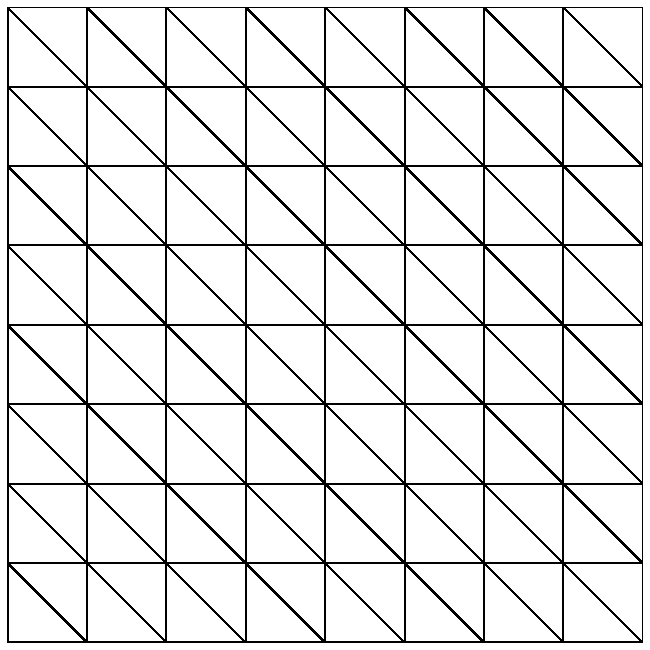
\includegraphics[width=\linewidth]{figures/interior_level0.pdf}\\[0.05em]
{\footnotesize L=0,\ ratio 1}
\end{minipage}%
\hspace{0.04\linewidth}%
\begin{minipage}{0.38\linewidth}
\centering
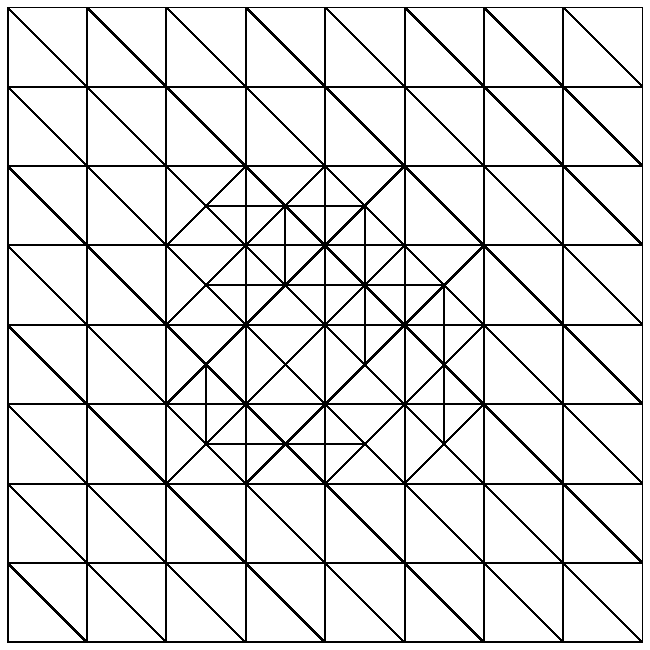
\includegraphics[width=\linewidth]{figures/interior_level2.pdf}\\[0.05em]
{\footnotesize L=2,\ ratio 2}
\end{minipage}

\vspace{0.1cm}

\begin{minipage}{0.38\linewidth}
\centering
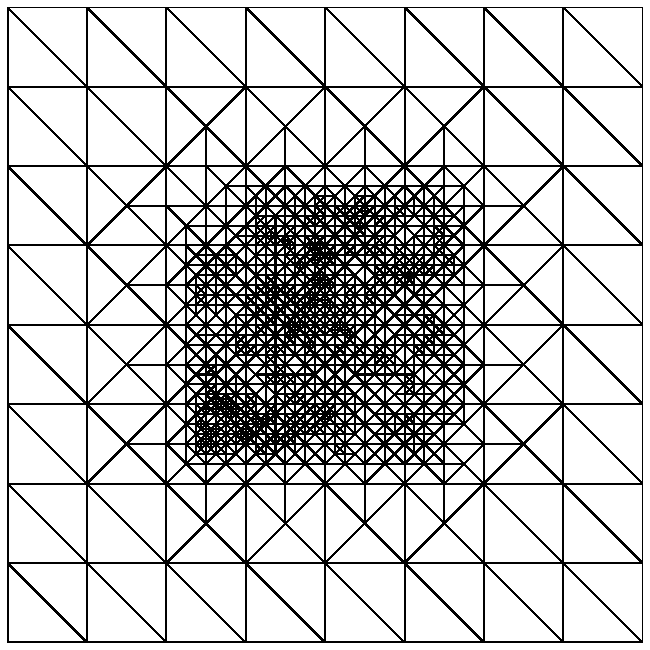
\includegraphics[width=\linewidth]{figures/interior_level8.pdf}\\[0.05em]
{\footnotesize L=8,\ ratio 16}
\end{minipage}%
\hspace{0.04\linewidth}%
\begin{minipage}{0.38\linewidth}
\centering
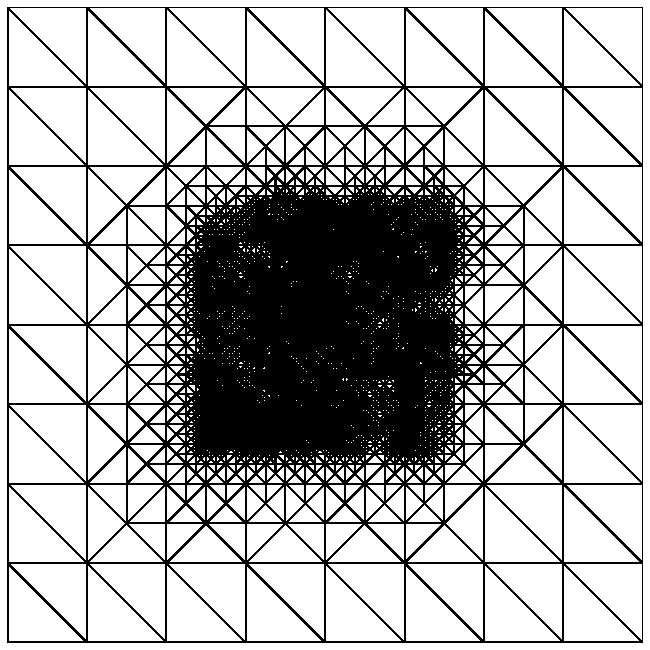
\includegraphics[width=\linewidth]{figures/interior_level12.pdf}\\[0.05em]
{\footnotesize L=12,\ ratio 64}
\end{minipage}
\end{block}

\end{column}

% ============= RIGHT COLUMN =============
\begin{column}{0.49\dimexpr\paperwidth-3cm\relax}

\begin{block}{Objectives}
\begin{enumerate}
\item \textbf{Check whether Schwedes' mesh dependence problem is still present} in the modern Firedrake, \texttt{pyadjoint}, and PETSc TAO stack, ten years on. Reproduce their experiment and determine which TAO solvers work correctly and which do not.
\item \textbf{Fix the mesh-dependence deeper in the solver.} Some optimisers solve a linear system inside every step, and that inner solve inherits the same mesh-dependence. Applying the Riesz map there too removes it - a contribution not covered by Schwedes.
\item \textbf{Deliver the fix as a \texttt{pyadjoint} feature.} Users should get correct mesh-independent behaviour from a single options entry, without needing to know about Riesz maps.
\end{enumerate}
\end{block}

\begin{block}{Reproducing the experiment (outer L-BFGS)}
\textbf{L-BFGS} is a widely-used quasi-Newton optimiser: it builds up a low-rank approximation of the Hessian across iterations and updates the solution using this approximation. Two L-BFGS optimisers run on the same problem, on the same mesh sequence, to the same tolerance. The only difference is the inner product each uses internally.

\vspace{0.3em}
\centering\small
\begin{tabular}{lrrrrrrrr}
\toprule
Inner product used & L=0 & L=2 & L=4 & L=6 & L=8 & L=10 & L=12 & L=14 \\
Realised $h_{\max}/h_{\min}$          & 1 & 2 & 4 & 8 & 16 & 32 & 64 & 128 \\
\midrule
Euclidean $\ell^{2}$                  & 13 & 39 & 71 & 104 & 205 & 401 & 701 & 1269 \\
Function-space $L^{2}$                & 6 & 8 & 6 & 8 & 7 & 8 & 8 & 6 \\
\bottomrule
\end{tabular}

\vspace{0.4em}
\justifying
The $\ell^{2}$ row grows nearly $100\times$ across the sweep, matching the polynomial dependence predicted by Schwedes. The $L^{2}$ row stays bounded between 6 and 8. TAO's \texttt{lmvm} solver reproduces the flat row once its default limited-memory history is raised from five to one hundred.
\end{block}

\begin{block}{Preconditioning}
Some iterative solvers, like \emph{conjugate gradient} (CG), can converge very slowly when the underlying matrix is badly conditioned. A \emph{preconditioner} $P$ transforms a difficult linear system $Ax = b$ into an easier one,
\[
P^{-1}Ax = P^{-1}b,
\]
whose matrix $P^{-1}A$ is close to the identity. The iterative method then converges much faster - often in a number of iterations independent of problem size. For the reduced Hessian on non-uniform meshes, the Riesz map $M_h^{-1}$ is exactly the right preconditioner: it cancels the cell-size scaling that would otherwise ruin the conditioning.
\end{block}

\begin{alertblock}{New result: preconditioning the inner CG of TAO/NLS}
TAO has many optimisers. L-BFGS (previous section) builds a Hessian approximation across iterations, so a correct choice of inner product is enough to make it mesh-independent, and it does not need a preconditioner. \textbf{NLS} (Newton Line Search) is Newton's method: at each outer step it solves the exact reduced-Hessian system for a search direction, using inner CG. On our test problem NLS takes only two outer iterations, but each inner CG grows in iteration count with mesh non-uniformity unless preconditioned. The discrete Riesz map $M_h^{-1}$ removes this growth completely.

\vspace{0.3em}
\centering
\begin{tikzpicture}
\begin{axis}[
  width=0.95\linewidth, height=7.5cm,
  xlabel={Realised $h_{\max}/h_{\min}$ (log scale)},
  ylabel={Inner-CG iterations (log scale)},
  xmode=log, ymode=log,
  log basis x=2, log basis y=10,
  xmin=0.9, xmax=160,
  ymin=8, ymax=1500,
  xtick={1,2,4,8,16,32,64,128},
  xticklabels={1,2,4,8,16,32,64,128},
  ytick={10,100,1000},
  yticklabels={10,100,1000},
  grid=major,
  grid style={line width=.2pt, draw=gray!30},
  major grid style={line width=.3pt, draw=gray!50},
  legend pos=north west,
  legend style={font=\small,draw=none,fill=none},
  every axis plot/.append style={line width=1.2pt, mark size=3pt},
]
\addplot[color=red!80!black, mark=*]
  coordinates {(1,24) (2,40) (4,65) (8,108) (16,197) (32,341) (64,610) (128,1111)};
\addlegendentry{no preconditioner ($\ell^{2}$)}
\addplot[color=ImperialBlue, mark=square*]
  coordinates {(1,10) (2,15) (4,14) (8,13) (16,13) (32,14) (64,13) (128,14)};
\addlegendentry{with $L^{2}$ Riesz PC ($M_h^{-1}$)}
\end{axis}
\end{tikzpicture}

\vspace{0.2em}
\justifying\small
The uncorrected inner solve inherits the same weakness as the outer optimiser: iteration counts grow nearly $50\times$ across the mesh sweep. The $L^{2}$ Riesz-map preconditioner does at the Krylov level what changing the inner product does at the optimiser level, restoring mesh-independence completely. This connection is pointed at by [3, Sect.~1.3.3] using [4], but it is not tested experimentally in the book.
\end{alertblock}

\begin{block}{Work plan}
\begin{itemize}
\item \textbf{Ship the fix as a \texttt{pyadjoint} feature.} Users should be able to enable the Riesz preconditioner with a single options entry; the inner product should be read off the Control. This is the main remaining goal.
\item \textbf{Extend to $H^{1}$ and other Hilbert spaces on the control}, and characterise when each Riesz map is the correct preconditioner.
\item \textbf{Extend mesh-independence across TAO's optimisers.} Newton and L-BFGS now behave correctly; others, such as \texttt{bqnls}, do not yet. Bringing the whole solver family in line lets TAO be used with confidence on function-space problems.
\end{itemize}
\end{block}

\begin{block}{References}
\footnotesize
\begin{itemize}\itemsep0.1em
\item[{[1]}] Rathgeber et al.\ (2016). Firedrake: automating the finite element method by composing abstractions. \textit{ACM TOMS} 43(3).
\item[{[2]}] Mitusch, Funke, Dokken (2019). dolfin-adjoint 2018.1: automated adjoints for FEniCS and Firedrake. \textit{JOSS} 4(38).
\item[{[3]}] Schwedes, Ham, Funke, Piggott (2017). \textit{Mesh Dependence in PDE-Constrained Optimisation}. SpringerBriefs.
\item[{[4]}] Kirby (2010). From functional analysis to iterative methods. \textit{SIAM Review} 52(2).
\end{itemize}
\end{block}

\end{column}

\end{columns}

% ============= Footer =============
\vfill
\begin{beamercolorbox}[wd=\paperwidth,leftskip=1.5cm,rightskip=1.5cm]{block body}
{\color{ImperialBlue}\rule{\dimexpr\paperwidth-3cm\relax}{1pt}}\\[0.2em]
\hbox to \dimexpr\paperwidth-3cm\relax{%
  {\color{ImperialBlue}\normalsize \;\;\;\;\;\;\;\;\;\;\;\;Imperial College London}%
  \hfill
  {\color{ImperialBlue}\normalsize MSc Summer Research Fair, July 2026}%
  \hfill
  {\color{ImperialBlue}\normalsize imperial.ac.uk}%
}
\end{beamercolorbox}

\end{frame}
\end{document}
